\documentclass[12pt,a4paper]{article} % document setting, articles do not allow chapters
\usepackage[english]{babel} % english spell-check
\usepackage[utf8]{inputenc} % allows the input of special characters from keyboard
\usepackage[T1]{fontenc}
\usepackage{lmodern} %load modern fonts
\usepackage{helvet} % lead helvetica font
\renewcommand{\familydefault}{\sfdefault} % without this helvetica does not work on linux
\usepackage{textcomp} % for text symbols such as (C)
\usepackage{siunitx} % for mathematical embedding with $

\AtBeginDocument{\renewcommand{\bibname}{References}} % change Bibliography to Reference in TOC
%\usepackage[super, numbers]{natbib} % include bibliography
%\bibliographystyle{unsrtnat} % order by appearance
\usepackage[compress]{natbib}
\bibliographystyle{apalike} % simple bibliography style % sudo texhash
%\bibliographystyle{plainnat}
\usepackage{hyperref} % allow printing URLs (here: for Bibliography)
\usepackage{cite}

\usepackage{graphicx} % include figures
\usepackage[labelfont=bf]{caption} % change figure caption to bold

\usepackage{titlesec} %change title style
\titleformat*{\section}{\normalsize\bfseries}
\titleformat*{\subsection}{\normalsize\itshape}

%\usepackage[mathlines]{lineno} % add line numbers
\usepackage{setspace} %for double spacing

\usepackage{booktabs}
\usepackage{makecell}

\author{Masumi Stadler}
\title{PhD Manuscript 1}

%%%%%%%%%%%%
% Document %
%%%%%%%%%%%%
\begin{document}
%\linenumbers

\setlength{\parindent}{0cm}
Title (max 150 char): DNA-RNA dynamics reveal bacterioplankton assembly processes along a terrestrial-aquatic continuum\\

Masumi Stadler\textsuperscript{1,*}, Paul A. del Giorgio\textsuperscript{1}\\

Affilitation:\\
(1) Groupe de Recherche Interuniversitaire en Limnologie (GRIL), D\'{e}partement des Sciences Biologiques, Universit\'{e} du Qu\'{e}bec \`{a} Montr\'{e}al, Montr\'{e}al, QC, Canada


Institutional e-mail addresses: MS (stadler.masumi@courrier.uqam.ca), PdG (del\_giorgio.paul@uqam.ca)\\

Running title (max 50 char): Microbial communities along a boreal terrestrial-hydrological continuum.\\

*Contact corresponding author: Masumi Stadler \\
E-mail: m.stadler.jp.at@gmail.com \\
Phone: +1 (514)297-5330 \\
Address: D\'{e}partement des Sciences Biologiques, Universit\'{e} du Qu\'{e}bec \`{a} Montr\'{e}al, Case Postale 8888, Succursale Centre-Ville, Montr\'{e}al, QC, H3C 3P8, Canada \\

Keywords: aquatic bacterial communities, bacterioplankton, terrestrial-aquatic continuum, ecosystem connectivity, boreal ecosystems, mass effects, environmental sorting, metacommunity, microbial assembly, rare biosphere, rank abundance\\

Author contributions: PdG designed the sampling, MS collected the data, MS analysed the data, MS and PdG discussed the results and wrote the manuscript.\\

\newpage

\doublespacing

%\begin{abstract}


%\end{abstract}


\setlength{\parindent}{1cm}
\section*{Introduction}
Since the 1880s, we are starting to grasp the intriguing variety of microbial physiological pathways and how they are involved in many elemental elemental cycling processes on a global scale \citep{Caumette2015}. The variety in physiological pathways has been hypothesised to arise from the vast taxonomic diversity that we observe around the globe. Microbial communities found outside of the petri-dish are inherently taxonomically diverse, with richness estimations that defy imagination \citep{Thompson2017, Louca2019}. Richness varies among ecosystems with highest taxonomic reservoirs found in soils and less so in comparably nutrient depleted aquatic ecosystems \citep{Thompson2017}. While descriptive approaches of richness and taxonomic composition is common in almost any environment imaginable, little do we actually understand how microbes assemble into these diverse communities \citep{Shade2017a, Shade2018}. Inherited from community ecology in macrobiology, microbial assembly processes have similarly been defined into four fundamental processes - selection, dispersal, diversification and drift - \citep{Vellend2010}, which can be characterised by their degree of determinism and stochasticity \citep{Zhou2017}. Recent popular statistical approaches aim to quantify each assembly process, however, it relies on an assumption that taxonomically related organisms have similar functional traits \citep{Stegen2013a, Stegen2015a}. Phylogenetic conservatism is a concept that has been handled with care within the macro-biologies \citep{Losos2008, Warren2008}, but should be a target of even stronger discussions in microorganisms where species definitions remain unclear \citep{Achtman2008} and genetic exchanges are common \citep{Thomas2005}. Indeed, many microbial traits have been shown to be phylogenetically conserved \citep{Martiny2015} but it was also noted that more complex traits encoded by many genes are more likely to be conserved while simpler traits that involve fewer genes are rather phylogenetically dispersed \citep{Martiny2013a}. It is also na\"{i}ve to assume that the ensemble of traits harboured in the genome are expressed in the environment at all times. Phenotypic variation with the same genotype due to differences in expression levels is indeed possible and common (e.g. epigenetics) \citep{Caumette2015}. Additionally, the increasing literature on potential niche segregation within the same species (i.e. ecotypes) \citep{VanRossum2020} exemplify intraspecies versatility that can blur patterns based on phylogenetic conservatism \citep{Achtman2008, Ackermann2015, Chase2018}. Thus, any inference on assembly based on taxonomy and/or phylogeny has to be interpreted with caution.

In concert with the lack of suitable approaches, traditionally, microbial community dynamics have been examined one ecosystem at a time. Most field studies, investigate the intriguing seasonal and spatial fluctuations of community composition within individual terrestrial, freshwater and marine ecosystems (hereafter ecosystem domains) \citep{Shigyo2019,Jones2012,Hassell2018,Giovannoni2012}. Even among freshwater studies, researchers tend to focus on either streams, lakes, or rivers \citep{Logue2008}. While this approach gives an in-detail insight into ecosystem specific community dynamics, it neglects an inherent characteristic of nature: connectivity beyond ecosystem boundaries.

Literature is scarce when searching for studies that cover multiple ecosystem domains within a study \citep{Nemergut2011, Shade2013} and it is even rarer to investigate multiple ecosystem domains that are physically connected \citep{Ruiz-Gonzalez2015, Hauptmann2016, Doherty2017}. Microorganisms without motility machineries are seemingly stationary, although being dispersal limited to a certain degree \citep{Hanson2012}, the miniscule size of microorganisms generally promotes dispersal. Within a watershed, freshwaters act as a carrier of matter, from the terrestrial milieu over freshwater networks to ultimately the ocean. Especially during strong rain events, freshwater flushes through the earth, extracting all soluble nutrients and capturing matter - dead or alive - along its hydrological evolution from a raindrop to collectively becoming a stream. On its further journey, the rushing water may be stopped by lakes and reservoirs that temporarily give more time for some organisms to thrive and previously unavailable resources may be degraded with longer hydraulic residence times \citep{Catalan2016a}. Within the aquatic network, dynamics in hydrology have been determined to be one of the major drivers of microbial community composition \citep{Nino-Garcia2016} and evidence suggests that a large proportion of aquatic microbial communities can be traced back to soils \citep{Crump2012, Besemer2013, Ruiz-Gonzalez2015, Hauptmann2016}. Different branches of the aquatic network collect taxa from all sub-catchments within a watershed, potentially creating sub-watershed specific unique communities at each sub-catchment's mouth. Thus, not every member within diverse communities at a single location shares a similar history in terms of origin \citep{Nino-Garcia2016, Comte2017} or reacts similarly to changing environmental conditions \citep{Fierer2007}. However, such passive dispersal implies that occurrence of a taxon in an unsuitable habitat merely by accident is also likely.

Death and dormancy \citep{Cole1999, Jones2010} questions the suitability of DNA approaches to study ecological 'communities'. In a strict ecological sense, a community refers to an assemblage of various species that interact with each other, sharing niches in forms of available space or resources \citep{Konopka2009}. However, DNA methods are not able to distinguish the actively participating from the passive members. Since, researchers have expanded their molecular toolbox to RNA approaches to capture taxa that have invested in protein synthesis in the recent minutes to hours \citep{Blazewicz2013}. Evidence of 16S rRNA has opened windows to study differential responses of the potentially active community to environmental variables and available resources \citep{Osterholz2016}. Being target of scrutiny and criticism, RNA may not be a good indicator of absolute growth or activity rates \citep{Blazewicz2013}, however, changes in RNA levels of the same taxa along gradients does imply a certain reaction of a taxon to environmental or biological changes. Thus, to this date, the full potential of RNA approaches in the context of microbial community assembly has yet to be explored.

In this study, we followed the Romaine river in North-Eastern Qu\'{e}bec, Canada, as an example watershed over several years and seasons. Our overall objective was to understand microbial succession and assembly processes along a terrestrial-hydrological continuum without any phylogenetic inference but rather simply by following and comparing the bulk DNA to the reactive RNA assemblages, respectively. Therefore, soils, soilwater, groundwater, streams, the river, lakes, reservoirs and the estuary were sampled for DNA and RNA and sequenced for the 16S rRNA gene to characterise the taxonomic composition of each fraction. We specifically wanted to explore firstly, whether we have distinct microbial communities depending on habitat types and if we can find seasonality across all ecosystems. We hypothesised that firstly, seasonality will be reflected in all communities of the different ecosystems as boreal climate zones do exhibit strong seasonality that is accompanied by shifts in available light, temperature and thus affect vegetation and aquatic and terrestrial bodies substantially. Secondly, we expected a gradual change in community composition along the continuum rather than distinct separate clustering of terrestrial and aquatic communities as we expect headwater streams to represent "ecotones" between terrestrial and larger aquatic water bodies due to their high connectivity to the surrounding terrestrial environment. Thirdly, we hypothesised that dynamics in DNA and RNA assemblage divergence and convergence enables us to grasp what dominating assembly process (i.e. mass effect and selection) is governing the community at a certain point in the continuum. And lastly, we wanted to explore where in a typical rank abundance curve (e.g. rare vs abundant taxa) community reshuffling is happening as the communities change habitats along the continuum.
%Furthermore, the consecutive flooding of three reservoirs over the sampled years created a unique opportunity to study the transformation process of a running system into a standing water body.
%(should be around 900~1000 words)

\section*{Material and methods}
\subsection*{Catchment characteristics and sampling design}
To follow the movement of microbial communities within a watershed, samples were taken along the Romaine river (C\^{o}te-Nord region, Qu\'{e}bec, Canada) (Fig. 1a-b) for three years from 2015-2017. The Romaine catchment belongs to the eastern black spruce-moss bioclimatic domain and drains an area (\textit{A}) of approximately 14 500 km\textsuperscript{2}.

The river springs between the Atlantic and Saint Lawrence watersheds (52\textdegree{}52'20"N 63\textdegree{}36'55"W; 702 masl), and consequently flows through a series of lakes (hereafter riverine lakes) including the biggest lake in the catchment – Lake Br\^{u}l\'{e} (\textit{A}: 127.11 km\textsuperscript{2}, elevation: 470 masl). The river mainly flows towards the South with a maximum distance from the northern headwaters to the river mouth expanding to approximately 475.1 km. Nearly half of the catchment is covered by coniferous forests (\textit{P.mariana}-moss), with mixed forests being rather minor (11\%) and deciduous stands with white birch (\textit{Betula papyrifera}) and trembling aspen (\textit{Populus tremuloides}) are even more rare (2\%)\citep{HQreport2009}.  A weather station located in the lower coastal plain (50\textdegree{} 16'55.000" N, 63\textdegree{} 36'41.000" W, Havre-Saint-Pierre Airport, Natural Resources Canada) recorded an annual precipitation of 810.77 $\pm$ 35.25 mm and 1.18 $\pm$ 0.73 \textdegree{}C, -32.63 $\pm$ 1.36 \textdegree{}C, and 25.8 $\pm$ 0.66 \textdegree{}C for mean, minimum and maximum temperature over the sampled years. More catchment characteristics are detailed in the supplementary methods (hereafter, SM).

The Romaine river has been dammed during the sampling period, forming a reservoir cascade complex with 4 reservoirs by 2020. The reservoirs Romaine 2 (RO2, \textit{A}: 81.15 km\textsuperscript{2}, mean depth 61 m), Romaine 1 (RO1, \textit{A}: 13.22 km\textsuperscript{2}, mean depth 22 m) and Romaine 3 (RO3, \textit{A}: 35.18 km\textsuperscript{2}, mean depth 66 m) were flooded in the years 2014 (winter), 2015 (winter), and 2017 (spring), respectively.

Overall, 395 samples were collected for DNA and 202 for RNA, covering spring (166:69, DNA:RNA), summer (195:99) and autumn (34:34). RNA samples were sampled from 2016 onwards. To follow a terrestrial-aquatic continuum various habitat types have been sampled (Table S1). Due to the remoteness and inaccessibility of the northern most headwaters, we sampled the Petite Romaine sub-catchment (PR, \textit{A}: 310.73 km\textsuperscript{2}, elevation: 580 masl, Fig. 1c) for streams and headwater ponds. This sub-catchment represents a headwater stream network in our studied continuum.

Surface soil samples were collected by mixing three randomly selected cores (30 cm) that were taken in proximity of installed piezometers to sample soil-water. The upper 5 cm including surface vegetation were removed before the soil was transferred into a sterile plastic bag. Three piezometers were randomly installed in proximity (30-100 cm) to a sampled stream with an average depth of 50 $\pm$ 20 cm. However, if the piezometers were installed too close to the stream main channel, hyporheic water was sampled instead. Piezometers were emptied 3 times (1-2 h) with a peristaltic pump before sample water was collected. The water from the randomly installed piezometers were pooled together. Groundwater was directly collected from constructed wells with submersible pumps. Surface water samples were directly collected into a pre-rinsed carboy bottle at a depth of 0.5 m, close to the shore for stream samples and diverse locations within the river and reservoirs. Lake sediment samples were collected with sediment cores (1-2 m depth), and the upper 10 cm were collected and mixed for subsequent processing. All samples were stored at 4 \textdegree{}C upon arrival at the laboratory until further processing on the same day of sampling.

\subsection*{Sample processing and sequencing}
Homogenised soil and sediment samples were transferred to aliquots of 0.25 g and frozen immediately on the same day of sampling. A minimum of 25 mL and 250 mL of soil-/hyporheic-water and surface water, respectively, was filtered through 0.22 \si\micro m polycarbonate membrane filters (Merck Millipore, Darmstadt, Germany), and subsequently stored frozen. All DNA and RNA samples were frozen at -20 \textdegree{}C at the field station and further stored at -80 \textdegree{}C at the university laboratory until extraction. Samples for RNA extraction were submerged in RNAlater\textsuperscript{\textregistered} and LifeGuard\textsuperscript{\textregistered} Soil Preservation solution (QIAGEN\textsuperscript{\textregistered}, Hilden, Germany) for water and humic samples (soil, soilwater, hyporheic water), respectively. To allow stabilisation in the buffer, samples were left at 4 \textdegree{}C overnight and were subsequently stored frozen.

Following the manufacturers instructions, PowerWater\textsuperscript{\textregistered} and PowerSoil\textsuperscript{\textregistered} DNA and RNA extraction kits (MoBio, Carlsbad, CA, USA) were used to extract water and soil/soil-/hyporheic-water/sediment samples, respectively. In 2017, the equivalent DNeasy\textsuperscript{\textregistered} and RNeasy\textsuperscript{\textregistered} PowerWater\textsuperscript{\textregistered} Kits (QIAGEN\textsuperscript{\textregistered}) were used for DNA and RNA samples, respectively, due to discontinuation of the kit series. RNA extracts were synthesized to cDNA (SM2) and all samples were sent to G\'{e}nome Qu\'{e}bec Innovation Centre (Montr\'{e}al, QC, Canada) for paired-end metabarcoding of the 16S rRNA V4 region using the primers 515F (5'-GTGCCAGCMGCCGCGGTAA-3') and 806R (5'-GGACTACHVGGGTWTCTAAT-3') on a Illumina MiSeq (PE250) platform.

\subsection*{Bioinformatic analysis}
A detailed description of the bioinformatic treatment can be found in the SM. In brief, primers were removed from 16S rRNA DNA and cDNA (hereafter RNA) reads using \textit{cutadapt} (Version 1.18, \citet{Martin2013}). To identify amplicon sequence variants (ASVs), 16S rRNA amplicon reads were analysed through the DADA2 (Divisive Amplicon Denoising Algorithm 2) pipeline (Version 1.14.1, \citet{Callahan2017}) on R Version 3.6.3 \citep{RCoreTeam2017}). All ASVs that are identical in sequence but differ only by length were merged together, leading to ASVs that represent a unit similar to 100\% similarity operational taxonomic units (OTUs) and chimeras were removed. Taxonomy was assigned with the \textit{DECIPHER} package (Version 2.14.0, \citet{Wright2016}) implementing the increased accuracy IDTAXA algorithm \citep{Murali2018} and the provided trained classifier of the SILVA database (Version 138, \citet{Pruesse2007}). Even after merging ASVs into 100\% OTUs, several ASVs were found to be highly abundant only in RNA. To account for slight differences that may have emerged between DNA and RNA ASVs and also to merge potential differences among 16S rRNA copies within a single genome, ASVs were merged into OTUs by a 99\% similarity threshold \citep{Vetrovsky2013} with the \textit{DECIPHER} package \citep{Wright2016}.

All OTU observations with less than 10 reads per sample were removed. Furthermore, \textit{metagenomeSeq} was used to transform and stabilise variation in library sizes with cumulative sum scaling (CSS) \citep{Paulson2013}. CSS results were rounded to its integer to represent count data (hereafter: CSS reads). CSS results were compared with results achieved with various rarefaction thresholds (see).

\subsection*{Data exploration and statistical analyses}
To explore differences in microbial community composition across habitat types and seasons, a Principal Coordinates Analysis (PCoA) was conducted with Bray-Curtis dissimilarities ($D_{BC}$) \citep{Bray1957, Legendre1998} based on all DNA samples with the function \textit{pcoa} in the \textit{ape} package \citep{Paradis2018}) (n = 372, 20185 OTUs). The community matrix was log transformed, (log\textsubscript{2}(x + 1)) to resolve a strong horse-shoe effect. The $D_{BC}$ matrix was square-root transformed to make the distance matrix Euclidean \citep{Legendre1998, Borcard2011}. A PERMANOVA was computed with 9999 permutations to evaluate statistical differences in habitat type and season  with the \textit{adonis} function in \textit{vegan} \citep{Oksanen2017}. The null hypothesis of this approach is that the cluster centroids do not differ between groups \citep{Anderson2013}. The test cannot distinguish among-group from within-group variation if data dispersion is variable among groups. Thus, an analysis of multivariate homogeneity was computed with \textit{betadisper} in \textit{vegan} \citep{Oksanen2017} by accounting for small and uneven sample sizes with the \textit{bias.adjust} argument. Using \textit{permutest} in \textit{vegan} \citep{Oksanen2017}, we tested whether dispersion is variable among groups. The null hypothesis is that the average within-group dispersion is equivalent in all groups \citep{Anderson2013}. For all statistical analyses, an $\alpha$ level of 0.05 was chosen prior to analysis.

Secondly, to evaluate whether sampled RNA communities were further different from the DNA assemblages, we performed a second PCoA ($D_{BC}$ with square-root transformation) with both DNA and RNA samples (n = 572, 20185 OTUs). Again, statistically different clusters were investigated with a PERMANOVA (9999 permutations), where habitat type, season and nucleic acid type (DNA vs. RNA) formed the clusters. The same framework explained above to check for dispersions was applied.

To examine how different DNA and RNA assemblages of the same sample are, the distance of each DNA-RNA sample pair within the PCoA ordination space was computed across \textit{n}-dimensional space:


\[ m(p,q) = \sqrt{(\mid p_{1} - q_{1} \mid)^2 + (\mid p_{2} - q_{2} \mid)^2 + \cdots + (\mid p_{n} - q_{n} \mid)^2}\]


where $p$ and $q$ represent DNA and RNA site scores, respectively, of each sample. $n$ is the maximum number of dimensions. We focused on the first axes that cumulatively explain 75 \% of the variation for each ordination (n\textsubscript{75\%}). This approach was implemented, as it was evident from the PCoA that essential variation within non-aquatic samples were captured outside the first three axes. The distance metric thus allows us to still capture a large proportion of the variance, while separating noise and miniscule variation that has been split upon further several hundred axes of the PCoA. With this approach, we were able to narrow down the dimensions from 571 to 186 for the Bray-Curtis PCoA. As a proof of concept that the computed distance extracts a proportion of the individual pair-wise dissimilarities, summation of the distances across all PCoA dimensions (571 axes) equals the initial pair-wise Bray-Curtis dissimilarities, which is the input matrix into the PCoA (Fig. S3). Thus, calculating the distance across a subset of axes extracts a proportion of the pair-wise dissimilarities captured by the selected axes.

To further gain insight into the processes shaping assemblage dissimilarities, we computed a PCoA with the S{\o}rensen dissimilarity ($D_{S}$), which is the incidence based equivalent of $D_{BC}$ (square-root transformed to achieve Euclidean space) \citep{Sorensen1948, Legendre1998}. We further applied the same framework of calculating the distance among DNA and RNA pairs across n\textsubscript{75\%} axes (m\textsuperscript{S}). Finally, we calculated a ratio between the S{\o}rensen and Bray-Curtis distance to see when incidence based dissimilarity is greater than abundance and vice versa (m\textsubscript{S}:(m\textsubscript{BC}). This framework allows us to understand what shifts within the community is causing DNA and RNA assemblages to diverge. When m\textsubscript{BC} turns smaller than m\textsubscript{S} (high m\textsubscript{S}:m\textsubscript{BC}), we have fewer shared OTUs among DNA and RNA, and abundance differences are comparably smaller (more similar in m\textsubscript{BC}). In contrary, when we have a higher number of shared OTUs and abundance differences are larger, m\textsubscript{S} will be smaller than m\textsubscript{BC} (low m\textsubscript{S}:m\textsubscript{BC}). These interpretations were statistically tested with a Kruskal-Wallis test (Fig. S4).

%Non-linear regressions were computed to test the hypothesis that DNA-RNA distances are a function of $\alpha$ diversity indices (Shannon-Wiener index and Pielou's evenness). Regressions were computed on the means of habitat types. The best fit of the relationship was evaluated by computing linear regressions and polynomials of second and third degrees. The best model was selected based on a higher adjusted R\textsuperscript{2}, low residual sum squares and if models were very similar the simpler model was chosen.

\subsection*{Abundance groups}
Abundance groups (e.g. abundant, moderate, rare) were defined based on the shape of rank abundance curves per habitat type.  Abundance thresholds are defined as the first and second moment of maximum acceleration along the rank abundance curve. This approach classified all OTUs with >= 47 CSS reads as abundant, < 47 and >= 5 CSS reads as moderate, and < 5 CSS reads as rare (details in SM).

As a second step, we defined OTUs into spatial abundance groups (spAGs) based on their DNA abundance in each sample (Table 1). In brief, we distinguish OTUs that are present everywhere (universal [AG], cosmopolitan) from those that can be absent in certain habitat types. Additionally, there are categories for OTUs with differing abundance (abundant, moderate, rare) and whether they change AGs between habitats (shifters).

To evaluate how spAGs are distributed among the habitat types, we computed weighted averages scores of each OTU for the DNA-RNA PCoA with the \textit{wascores} function in \textit{vegan} \citep{Oksanen2017}. These species scores represent optima of each OTU within the PCoA ordination.\\[.3cm]

The packages \textit{phyloseq}, \textit{tidyverse}, \textit{plyr} and \textit{data.table} were used for data wrangling and transformation \citep{McMurdie2013,Wickham2019, Wickham2011, Dowle2019}, and \textit{doMC} and \textit{parallel} enabled parallel processing \citep{Analytics2019, RCoreTeam2017}. \textit{ggplot2}, \textit{ggpubr}, \textit{ggnewscale} and \textit{cowplot} were used to visualise the results \citep{Wickham2016, Kassambara2018, Campitelli2020, Wilke2019}. For statistical analyses, \textit{vegan} and \textit{rstatix} were used \citep{Oksanen2017, Kassambara2020}. All analyses have been conducted in R v3.4.2 \citep{RCoreTeam2017} and RStudio v1.3.1073 \citep{RStudioTeam2016}. Maps were created with QGIS (version 3.12) and a digital elevation model provided by Natural Resources Canada. Watersheds were delineated with ArcMap (version 10.5.1, ESRI Inc., Redland, CA) and the Spatial Analyst Toolbox.

\section*{Results}
Sampled sites covered a large range of habitat types from soils, soilwater, over streams, the main river, lakes, reservoirs and the estuary. We recovered 87 002 470 quality reads, with 156 347 identified ASVs. There were 56 107 unclassified ASVs that were removed in the downstream analyses. After sub-sampling and 99 \% similarity clustering, 47 402 282 reads and 20 220 OTUs were retained. The smallest and largest library size were both found in riverine lakes with 2851 and 1 333 391 reads, respectively. On average, the lowest library sizes were found in sediments, soil and soilwater with less than 30 000 reads. In contrast, most freshwater samples had a library size higher than 50 000 reads (Fig. S6). 33 phyla, 80 classes,  189 orders, 400 families, and 696 genera were represented in the dataset. Relative abundances of phyla varied across habitat types (Fig. S6) but on average, the meta-community across all ecosystems was composed of 52.11 \% Proteobacteria, 17.17 \% Actinobacteria, 8.06 \% Verrucomicrobiota, 6.88\% Bacteroidota, 2.91 \% Acidobacteriota, 2.63 \% Planctomycetota, 2.37 \% Cyanobacteria, 1.43 \% Myxococcota, 1.23 \% Desulfobacterota, 1.22 \% Chloroflexi and 1.19 \% Nitrospirota.

\subsection*{Gradual change of DNA assemblages along a terrestrial-aquatic continuum}
We observed a gradual separation of terrestrially-influenced habitats such as soil, soilwater and sediment from freshwater and estuary samples along the first PCoA axis capturing 14.64 \% of the variance (Fig.2a). This observation was supported by the PERMANOVA analysis (\textit{F}\textsubscript{12} = 17.09, \textit{R}\textsuperscript{2} = 0.35, \textit{p} = 0.0001). Streams, groundwater, tributaries, headwater ponds, and lakes were creating a gradient between the two very distinct clusters of terrestrial and riverine/reservoir samples (Fig.2a).

The trajectory along the continuum has a striking seasonality where spring and summer/autumn samples cluster most pronounced in the reservoir samples along the second PCoA axis capturing 3.6 \% of the variance (PERMANOVA: \textit{F}\textsubscript{2} = 11.08, \textit{R}\textsuperscript{2} = 0.038, \textit{p} = 0.0001). Soil, sediment, soilwater and groundwater samples, however, do not exhibit a clear seasonality (Fig.2b). Seasonality does not emerge as a strong driver even within a PCoA performed only with terrestrial samples (Fig. S7). It is striking how seasonality takes effect as soon as we enter the streams and headwater ponds, where spring samples gradually form a path towards the spring riverine and reservoir cluster. In contrast to spring, streams do diverge faster from the terrestrial cluster and mingle more with other freshwater samples in summer and autumn. Interestingly, lakes are located in general more within the summer/autumn trajectory. These lakes, however, are not part of the continuum but were sampled across the watershed and thus are rather a part of the extended meta-community. Similarly, sediment samples cluster in the summer/autumn path without a single case lying in the spring trajectory.

A unique characteristic of the studied continuum is the addition of reservoirs over the sampled years. While the river fraction upstream of the reservoir (Upriver) has the same upstream history over the years, the continuum that feeds into the downstream of the reservoir (Downriver) changes over the years. In 2015, the downriver sites capture water from one reservoir (RO1), while in 2016 they feed from two reservoirs (+RO2, Fig. 1c). While in summer, there is no clear segregation, we can identify two distinct clusters in spring. Upriver and downriver sites are clustered separately in 2016, while in 2015 the furthest downriver sites closer to the river mouth converge back to the upriver sites (Fig. 2c, 2017 spring was not sampled).

Finally, estuary samples exhibit similar seasonality as reservoirs and rivers, however, the further one moves away from the river mouth, the estuary community gradually converges back along the first and second PCoA axis towards the centre of the ordination (Fig. 2d). At the furthest site from the river mouth, the estuary community in spring seems to share community members with stream and headwater pond samples in summer.

Although PERMANOVA results strongly supported habitat type and seasonal clustering, the results could be affected by different dispersion of data. Differential levels of dispersion was found by habitat type alone (PERMDISP: \textit{F}\textsubscript{12} = 32.17, \textit{p} = 0.0001), by solely season (PERMDISP: \textit{F}\textsubscript{2} = 42.79, \textit{p} = 0.0001) and by both habitat and season combined (PERMDISP: \textit{F}\textsubscript{27} = 17.77, \textit{p} = 0.0001). Although non-homogeneity of dispersion confounds a clear conclusion based on statistical evidence that habitat type and seasons are major drivers, ordination results indicate a very apparent difference in habitat type and seasonal microbial communities. It is also an interesting finding, that dispersions vary among habitat types and seasons. While dispersion between spring and summer was not statistically different (Tukey HSD: p > 0.05), they were always different when comparing autumn with other seasons (Tukey HSD: p < 0.0001). The average distance of samples within the autumn cluster to its median was smaller compared to other seasons (0.48 vs 0.62). Smaller variation in autumn likely emerges due to the fact that autumn was only sampled in one year, compared to spring and summer being sampled at least in two years. For habitat types, strong significant differences were most pronounced between soil/soilwater/stream samples with reservoir and river samples (Tukey HSD: p = 0). In general, within habitat type dispersion was larger in terrestrial samples (PERMDISP mean average distance to median: 0.6032), compared to riverine (0.5033) and reservoir (0.5124) samples. Indicating that terrestrial samples are more variable than freshwater samples. Within freshwater samples, there is a gradient in variance within stream, headwater ponds, lake and tributary clusters having highest dispersion levels close to terrestrial samples. Riverine, reservoir and estuary samples exhibited lowest dispersion with distances to the median centroid ranging between 0.39 to 0.49. One has to note here that both PERMANOVA and PERMDISP calculate the differences in factors across all PCoA axes. The visualised two axes capture most of the variance in the reservoir and riverine samples, thus they appear to be more variable. However, the variance of terrestrial samples seems to be spread over multiple axes and thus the cumulative dispersion across all dimensions results in higher values.

\subsection*{Clear divergence of aquatic RNA from DNA}
When DNA and RNA samples were combined, the second PCoA analysis captured in summary 19.85 \% of the dissimilarity variance in the first three axes, delineating habitat type (PC1), nucleic acid type (PC2) and seasons (PC3)(Fig.3). PERMANOVA analysis indicated significant clustering by habitat type (\textit{F}\textsubscript{12} = 20.65, \textit{R}\textsuperscript{2} = 0.29, \textit{p} = 0.0001), season (\textit{F}\textsubscript{2} = 14.86, \textit{R}\textsuperscript{2} = 0.35, \textit{p} = 0.0001) and nucleic acid type (\textit{F}\textsubscript{1} = 26.07, \textit{R}\textsuperscript{2} = 0.03, \textit{p} = 0.0001). Similarly to the DNA PCoA, homogeneity of dispersion was mostly not fulfilled. According to PERMDISP, dispersion differed by all factorial combinations (\textit{F}\textsubscript{48} = 10.96, \textit{p} < 0.0001), habitat type (\textit{F}\textsubscript{12} = 31.58, \textit{p} = 0.0001) and season (\textit{F}\textsubscript{2} = 44.26, \textit{p} = 0.0001), however, not for nucleic acid type (\textit{F}\textsubscript{1} = 1.65, \textit{p} = 0.12).

Overall, the PCoA's first three axes indicate that there is a very substantial seasonality in freshwater samples in both DNA and RNA. A similar seasonal and nucleic acid type dissimilarity to freshwater samples cannot be observed in terrestrially influenced samples (Fig. S7) and the strong seasonality in aquatic samples is captured in a PCoA only with RNA samples as well (Fig. S8). However, it is noteworthy that there were 29 axes with eigenvalues above 1, together summing up to 43.1 \% of the variance. Visual inspection indicated that a lot of the terrestrially influenced samples' dissimilarity was indeed split upon these additional axes, a clearer separation of soil and soilwater samples for example was observed in axes 6 (1.75\%), 10 (1.12\%), 11 (1.06\%) and 12 (0.99\%)(data not shown). However, apparent seasonality and large differences in nucleic acid type was not observed. Due to the high number of samples in this study, the PCoA resulted in 571 axes (n - 1) and thus the examined three axes only capture 19.85 \% of the overall variance that seems to capture the terrestrial-aquatic differentiation and seasonality within aquatic communities.

\subsection*{DNA and RNA mismatch patterns along the continuum}
To further explore the patterns in DNA-RNA differences along the continuum, we calculated the distance in ordination space between DNA and RNA of each sample (m\textsubscript{BC}) along the axes capturing 75\% of the variance as the depicted axes in Fig. 3 only capture aquatic DNA-RNA divergence. In spring, we can observe the largest differences in DNA-RNA in soilwater, followed by a gradual convergence between DNA and RNA along the continuum (Fig. 4a). This pattern is not reflected in summer and autumn, where the overall dissimilarity between DNA and RNA remains relatively similar across ecosystems. It is noteworthy, that outside of the direct continuum, tributaries and the riverine lakes located closer to the headwaters have a similar range in DNA-RNA divergence to soilwaters in spring. This DNA-RNA divergence in tributaries and riverine lakes cannot be observed in other seasons.

In order to focus on solely species identity differences between DNA and RNA, we further examined the distance in PCoA ordination computed with the S{\o}rensen dissimilarity (m\textsubscript{S}) which is solely based on incidences (i.e. presence-absence). m\textsubscript{S} indicates that the fraction of shared taxa between DNA and RNA increases along the continuum with the highest discrepancies in soilwater and streams (Fig. 4b). The decrease in m\textsubscript{S} along the continuum is more steep compared to m\textsubscript{BC}. Similarly to m\textsubscript{BC}, spring tributary and riverine lakes seem to exhibit similar magnitudes of DNA-RNA discrepancies.

In order to examine, when dissimilarities are driven more strongly by a shift in shared taxa identities or abundance discrepancies, we compared m\textsubscript{BC} with m\textsubscript{S}. When examinig the m\textsubscript{S}:m\textsubscript{BC} ratio along the contiuum we can observe a gradual decline in m\textsubscript{S}:m\textsubscript{BC} from soilwaters to the upriver indicating that there are in general fewer shared OTUs among DNA and RNA, and furthermore a higher similarity in DNA and RNA abundance. Subsequently, starting with the upriver summer, the following downstream ecosystems have a tendency to converge towards 1 and even fall below the 1:1 threshold. This pattern could indicate that with higher residence times, such as reservoirs and estuaries there are a higher number of shared OTUs among DNA and RNA, but there are larger discrepancies in their DNA and RNA abundances. A mismatch in abundance seems to be more prevalent in summer and autumn. Within the extended meta-community, most ecosystems have a tendency of higher m\textsubscript{S}:m\textsubscript{BC} ratios, with only riverine lakes in summer and other watershed lakes in autumn to have a small m\textsubscript{S}:m\textsubscript{BC}.

\subsection*{Community shifts along the rank abundance curve}
In order to understand where within a rank abundance curve, the observed community shifts are happening we calculated the DNA and RNA abundance difference and examined their relationship to m\textsubscript{BC}(Fig. 5a). It seems that in general community reshuffling is happening across all abundance groups, while a few abundance groups do contribute stronger than others with lower shifters being the most dynamic and large contributor to the observed DNA and RNA differences. Interestingly, lower m\textsubscript{BC} (e.g. < 0.6) seem to have minor DNA:RNA differences in rare and specialist OTUs, while moderate, lower shifters, cosmopolitans, and general shifters seem to contribute more substantially. In the extremest cases of m\textsuperscript{BC} > 0.8, the prior mentioned slight contributors, which are rare, specialist and upper shifters, increase their discrepancies as well. Overall, it seems that moderate and lower shifters have the highest variations in terms of their DNA and RNA abundances, which contributes to the divergence of DNA and RNA assemblages. Additionally, shifters and cosmopolitans steadily contribute to drifting DNA and RNA as well.

When examining the optima of each OTU within the first three PCoA axes (Fig. 5b), it becomes evident that overall, many rare and specialist taxa have their optima in terrestrial samples, while depending on the OTU, moderate, cosmopolitans and shifters can have optima in either aquatic or terrestrial habitats. While lower shifters do not necessarily have a strong pattern in ecosystem preference, they do have a tendency towards an optimum in RNA, compared to all other spatial abundance groups that lean towards DNA. In terms of seasons, only cosmopolitans seem to have optima in spring, while most other spAGs lean towards summer and autumn.

\section*{Discussion}

 %A potential driver of interannual differences are annual variations in hydrology. However, for 2015 and 2016, monthly total precipitation did not substantially vary in spring with 77.5 $\pm$ 5.51 mm in April, 67.4 $\pm$ 4.24 mm in May, 123.2 $\pm$ 13.72 mm in June. However, daily precipitations had a higher variance in June 2016 compared to 2015.

 %Criticism has arised to use RNA of the 16S rRNA gene to infer activity of microorganisms out of concern that several biases may obscure adequate interpretations. The main concerns circle around evidence of multiple 16S copy numbers within different microbial genomes (xx) and differing biases introduced between DNA and RNA preparation and sequencing approaches that make DNA:RNA ratios of individual taxa difficult to interpret. Nevertheless, it is a premature decision to completely abandon 16S rRNA RNA approaches before exploring all potential applications.

\subsection*{Data accessibility}
The raw 16S rRNA gene seqeuences, both DNA and cDNA are available at the public NCBI Sequence Read Archive (SRA) under the accession numbers SRxxxxx. The code and meta data that were used to produce this manuscript are available at \url{https://github.com/CarBBAS/xxx} (Zenodo DOI). (Links, accession numbers and DOI will be updated upon acceptance) \\

\section*{Conflict of Interest}
The authors declare no conflict of interest.

\section*{Acknowledgements}
We are especially grateful to Alice H. Parkes, Annick St-Pierre, and Serge Paquet, who maintained and oversaw the La Romaine project over the years. Collection and analysis of all variables would have not been possible without the support from members of the CarBBAS team including great contributions from undergraduate students. Therefore, we would like to thank Felipe Rust, Clara Ruiz-Gonz\`{a}lez, Trista Vick-Majors, Alexandre Ducharme, Roy Nahas, Ryan Hutchins, Marie Laure G\'{e}rardin,  Erin Hotchkiss, Karelle Desrosiers, Martin Demers, Sara Mercier Blais, Julia Jakobsson, Francesca del Giorgio, Brenden Chabot, Sebastian Dugas, and Pascale Ouimet. We would also like to thank Katherine Velghe and Marilyne Robidoux for laboratory assistance, Mario Muscarella for insightful discussions and Robert Ptacnik and Yves Prairie for statistical advice. We also thank xx anonymous reviewers for constructive comments that improved the manuscript. This study is part of the program of the Carbon Biogeochemistry in Boreal Aquatic Systems (CarBBAS) Industrial Research Chair, co-funded by the Natural Science and Engineering Research Council of Canada (NSERC) and Hydro-Qu\'{e}bec.

\newpage
\singlespacing

\bibliography{/media/shared/Documents/University/PhD/BibTEX/LR_miccom_paper}

\newpage
\section*{Figure legends}
Figure 1. \textbf{Location and overview of the La Romaine catchment}. a) Scale and overview of the whole La Romaine catchment. Samples are represented as points. b) Location of the catchment within Canada and Québec. c) Focus on all built reservoirs RO1 (2015), RO2 (2014) and RO3 (2017) and the headwater stream sub-catchment Petite Romaine (PR).\\
\\
Figure 2. \textbf{Microbial community composition gradually changes along a terrestrial-hyrodlogical continuum and diverges between seasons.} Overall PCoA analysis of DNA samples (a) has been further explored with focus plots on terrestrial, riverine and estuary samples in panels b, c, d, respectively. Overall, the PCoA reveals microbial community shifts from terrestrial to freshwater samples. Spring and summer-autumn show distinct paths in multivariate space. Habitat types are indicated in colours, and shapes differentiate seasons. Percentage of variance explained are given in square brackets for the first and second axis. \\
\\
Figure 3. \textbf{RNA assemblages diverge from DNA within aquatic habitats, less so in terrestrially influenced habitats.} PCoA analysis inclduing RNA samples. a) Visualisation of first and second axis of PCoA, differentiating habitat type and nucleic acid type, respectively. b) Different view on PCoA analysis using the second and third axis, differentiating nucleic acid type and seasons, respectively. Seasons are given in different point shapes, colouring visualises different habitat types, opacity indicates nucleic acid type. Percentage of variance explained are given in brackets for the first, second and third axes. \\
\\
Figure 4. \textbf{RNA assemblages diverge from DNA within aquatic habitats, less so in terrestrially influenced habitats.} PCoA analysis including RNA samples. a) Visualisation of first and second axis of PCoA, differentiating habitat type and nucleic acid type, respectively. b) Different view on PCoA analysis using the second and third axis, differentiating nucleic acid type and seasons, respectively. Seasons are given in different point shapes, colouring visualises different habitat types, opacity indicates nucleic acid type. Percentage of variance explained by the corresponding axes are given in square brackets. \\
\\
Figure. 5 \textbf{Distance between DNA and RNA samples within PCoA ordination space reveals sections within the continuum that are dominated by species sorting or mass effects.} a) Distance based on Bray-Curtis dissimilarity (\textit{m}\textsubscript{BC}) among DNA and RNA assemblages of the same sample within the axes capturing 75 \% of the variance in PCoA. b) Ratio between distance calculated based on PCoAs computed with S{\o}rensen (\textit{m}\textsubscript{S}) and Bray-Curtis dissimilarity (\textit{m}\textsubscript{BC}). Points indicate the arithmetic mean and error bars represent standard deviations from the mean. Sample sizes of each point are indicated above in the corresponding colours. Sample sizes are equivalent in panels a and b. \\
\\
Figure 6.\textbf{DNA and RNA dissimilarities arise through abudance differences across the rank abundance curve.} a) Difference in DNA and RNA abundance against \textit{m}\textsubscript{BC}. Lines represent rolling means with bin size = 10. b) Boxplots and violin plots showing the distribution of species scores and thus OTU optima within PCoA space. The middle line represents the median, lower and upper hinges of boxplots correspond to the 25th and 75th percentiles. Upper and lower whiskers expand to the largest and smallest value, respectively, but no further than 1.5 times the inter-quartile range from the hinge. There were a plethora of outliers that lie beyond the whiskers for all boxes and thus, were removed for visualisation purposes. Violin plots visualise the probability density distribution smoothed by a kernel density estimator. \\

\section*{Tables}

\begin{table}

\caption{\label{tab:}Abundance groups}
\centering
\resizebox{\linewidth}{!}{
\begin{tabular}[t]{llr}
\toprule
Abundance groups & Criteria & Categorized OTUs\\
\midrule
Universal abundant & Abundant* in all habitats, never absent & 0\\
Universal moderate & Moderate* in all habitats, never absent & 0\\
Universal rare & Rare* in all habitats, never absent & 0\\
\addlinespace
Abundant & Only abundant observations, can be absent & 1\\
Moderate & Only moderate observations, can be absent & 4\\
Rare & Only rare observations, can be absent & 17459\\
\addlinespace
Specialist & \makecell[l]{Only abundant in one habitat type, \\ never abundant in any other habitats} & 1561\\
\addlinespace
Cosmopolitan & \makecell[l]{Shifts between abundant, moderate and rare, \\but present in all habitats} & 46\\
Shifter & Shifts between abundant, moderate and rare\textsuperscript{\dag} & 342\\
\addlinespace
Upper shifter & \makecell[l]{Shifts in the upper fraction (abundant - moderate) \\of the rank abundance curve\textsuperscript{\dag}} & 755\\
Lower shifter & \makecell[l]{Shifts in the lower fraction (moderate - rare) \\of the rank abundance curve\textsuperscript{\dag}} & 17\\
\bottomrule
\multicolumn{3}{l}{\rule{0pt}{1em}\textsuperscript{*} Abundant: 47 >= CSS reads, Moderate: 5 >= CSS reads < 47, Rare: 0 > CSS reads < 5} \\
\multicolumn{3}{l}{\rule{0pt}{1em}\textsuperscript{\dag} Does not have to be present in all habitats}\\
\end{tabular}}
\end{table}


\newpage

\section*{Figures}
\begin{figure}[!ht]
\centering
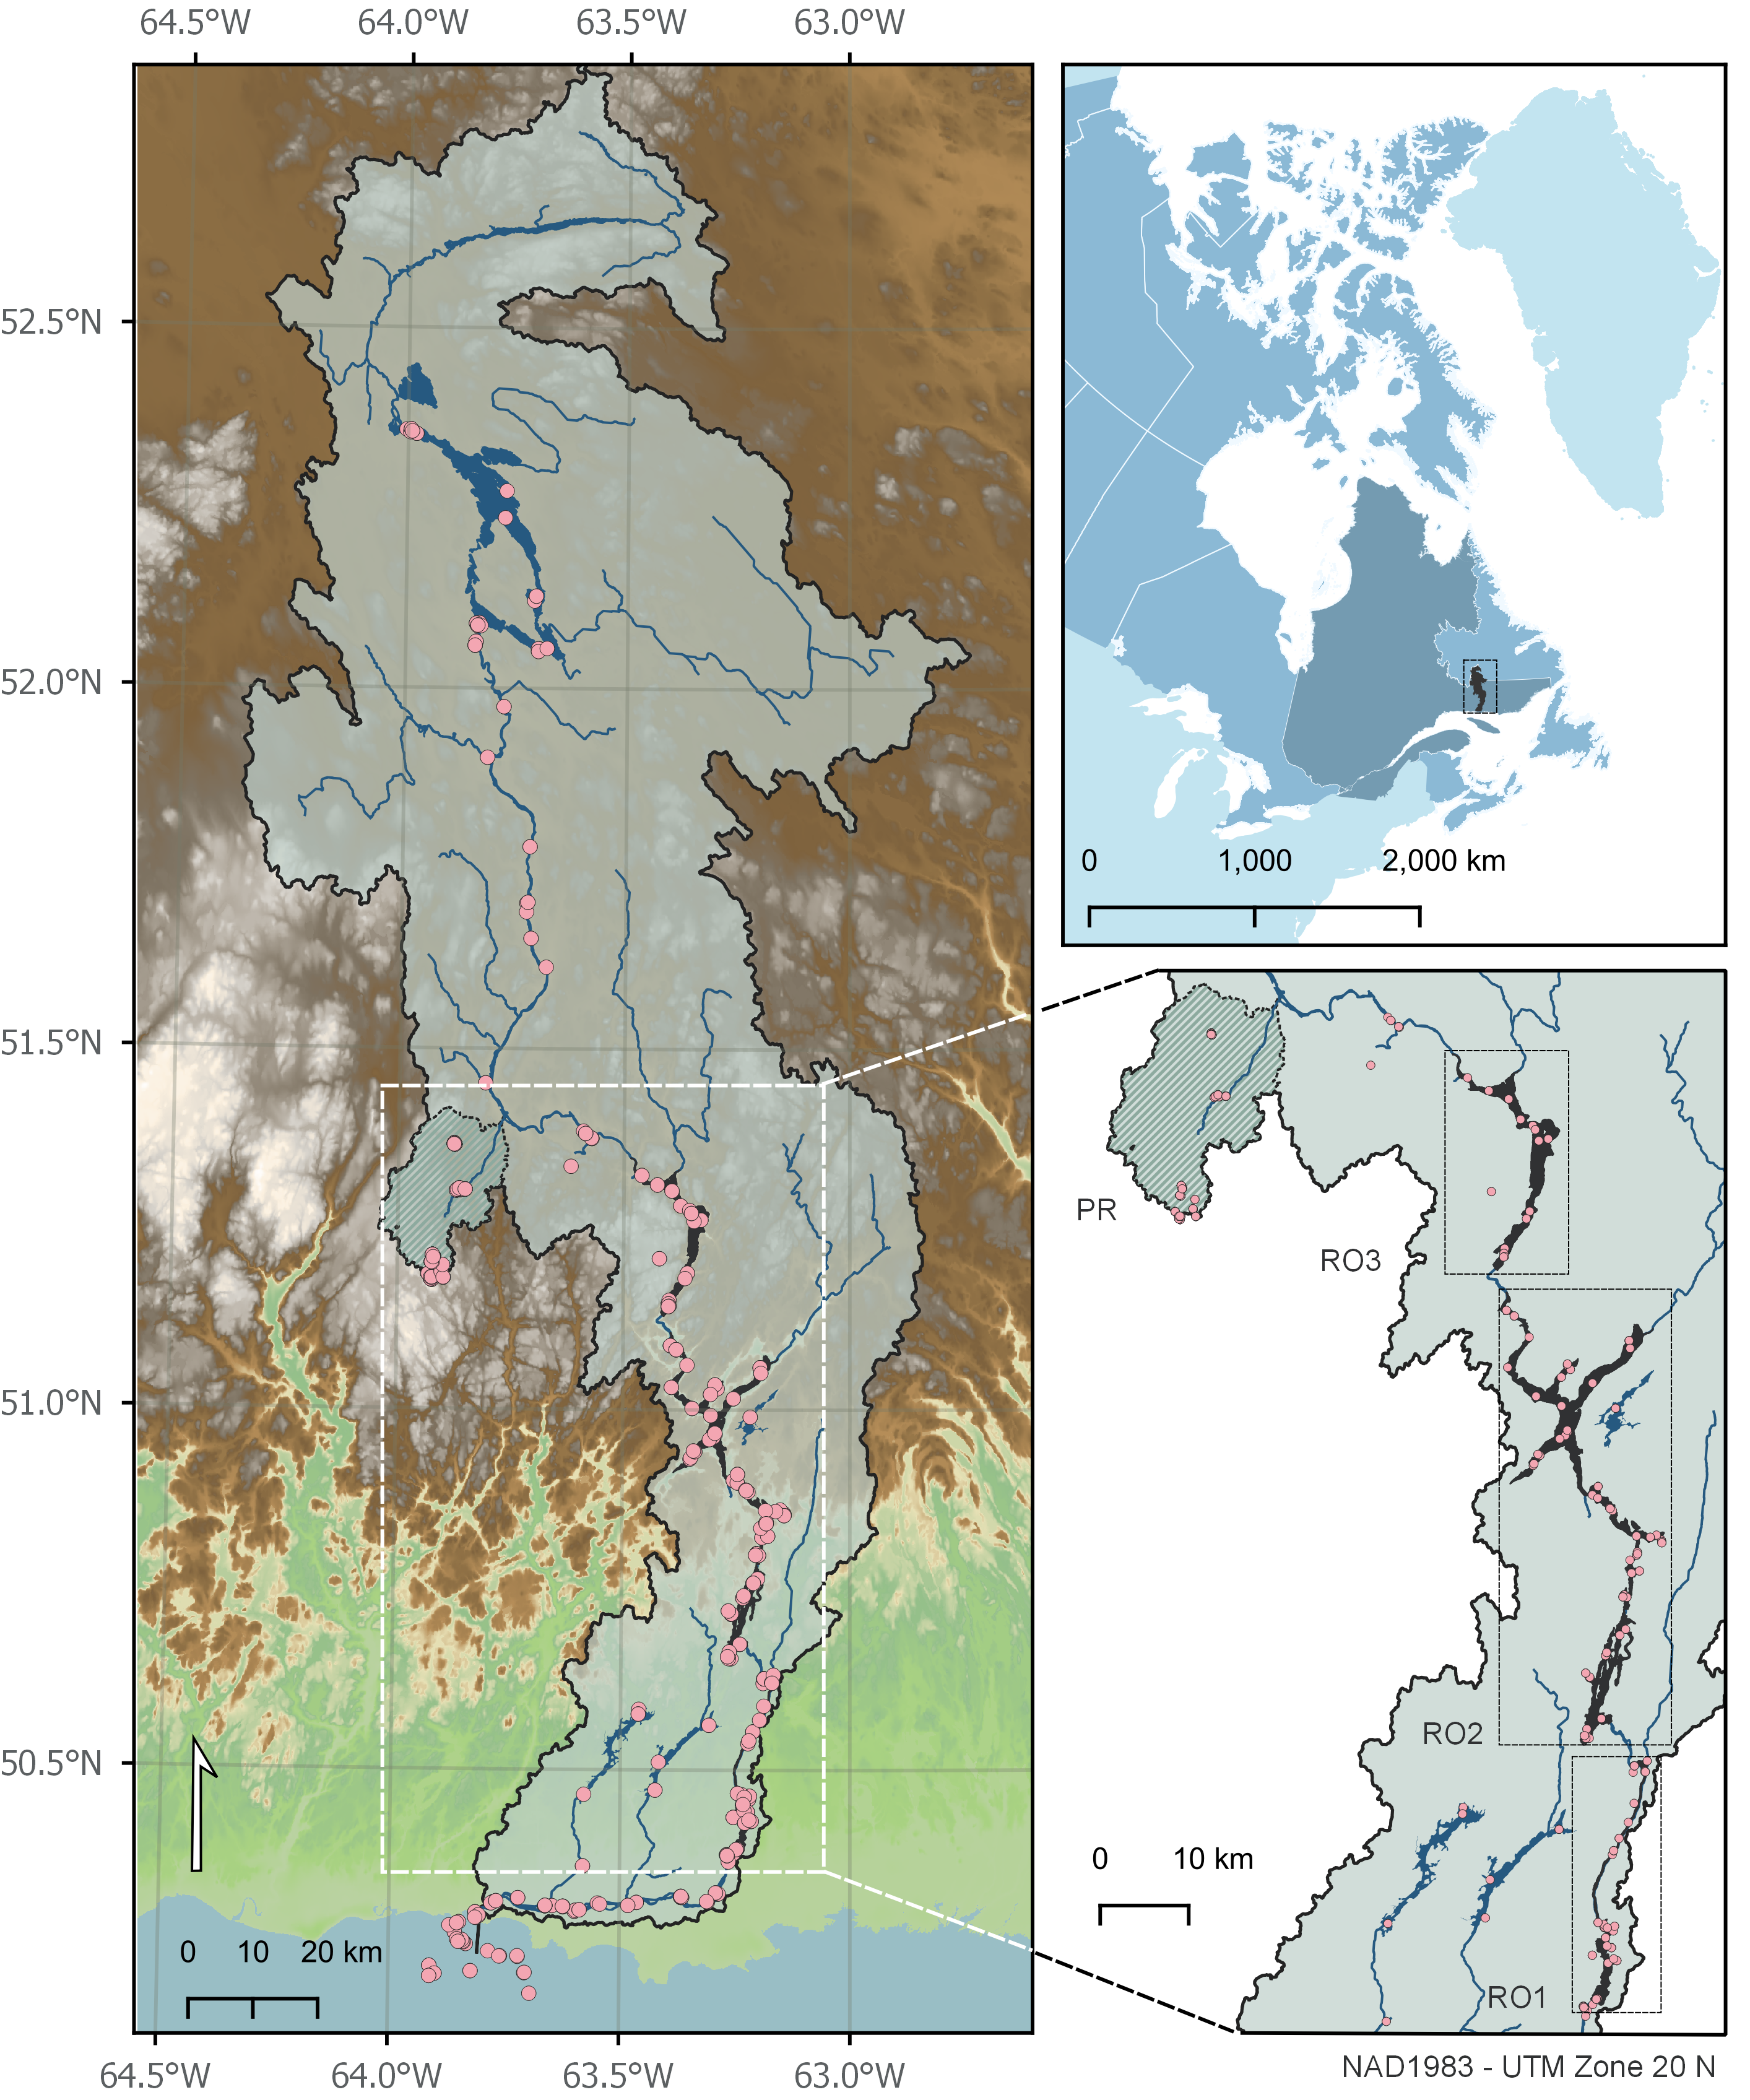
\includegraphics[width=12cm]{../Figures/LR_miccom_paper_threemaps.png}
\caption{\textbf{Location and overview of the La Romaine catchment}. a) Scale and overview of the whole La Romaine catchment. Samples are represented as points. b) Location of the catchment within Canada and Québec. c) Focus on all built reservoirs RO1 (2015), RO2 (2014) and RO3 (2017) and the headwater stream sub-catchment Petite Romaine (PR).}
%includegraphics[width=1\textwidth]
\end{figure}

\begin{figure}[!ht]
\centering
\includegraphics[width=16cm]{../../Figures/Final/PCoA_log_DNA_collage.png}
\caption{\textbf{Microbial community composition gradually changes along a terrestrial-hyrodlogical continuum and diverges between seasons.} Overall PCoA analysis of DNA samples (a) has been further explored with focus plots on terrestrial, riverine and estuary samples in panels b, c, d, respectively. Overall, the PCoA reveals microbial community shifts from terrestrial to freshwater samples. Spring and summer-autumn show distinct paths in multivariate space. Habitat types are indicated in colours, and shapes differentiate seasons. Percentage of variance explained are given in square brackets for the first and second axis.}
%includegraphics[width=1\textwidth]
\end{figure}

\begin{figure}[!ht]
\centering
\includegraphics[width=17cm]{../../Figures/Final/PCoA_all_SampleType.png}
\caption{\textbf{RNA assemblages diverge from DNA within aquatic habitats, less so in terrestrially influenced habitats.} PCoA analysis including RNA samples. a) Visualisation of first and second axis of PCoA, differentiating habitat type and nucleic acid type, respectively. b) Different view on PCoA analysis using the second and third axis, differentiating nucleic acid type and seasons, respectively. Seasons are given in different point shapes, colouring visualises different habitat types, opacity indicates nucleic acid type. Percentage of variance explained by the corresponding axes are given in square brackets.}
%includegraphics[width=1\textwidth]
\end{figure}

\begin{figure}[!ht]
\centering
\includegraphics[width=15cm]{../../Figures/Final/distBC_distratio_scat.png}
\caption{\textbf{Distance between DNA and RNA samples within PCoA ordination space reveals sections within the continuum that are dominated either by species sorting or mass effects.} a) Distance based on Bray-Curtis dissimilarity (\textit{m}\textsubscript{BC}) among DNA and RNA assemblages of the same sample within the axes capturing 75 \% of the variance in PCoA. b) Ratio between distance calculated based on PCoAs computed with S{\o}rensen (\textit{m}\textsubscript{S}) and Bray-Curtis dissimilarity (\textit{m}\textsubscript{BC}). Points indicate the arithmetic mean and error bars represent standard deviations from the mean. Sample sizes of each point are indicated above in the corresponding colours. Sample sizes are equivalent in panels a and b.}
%includegraphics[width=1\textwidth]
\end{figure}

\begin{figure}[!ht]
\centering
\includegraphics[width=15cm]{../../Figures/Final/abgroups_rollmean_violin}
\caption{\textbf{DNA and RNA dissimilarities arise through abudance differences across the rank abundance curve.} a) Difference in DNA and RNA abundance against \textit{m}\textsubscript{BC}. Lines represent rolling means with bin size = 10. b) Boxplots and violin plots showing the distribution of species scores and thus OTU optima within PCoA space. The middle line represents the median, lower and upper hinges of boxplots correspond to the 25th and 75th percentiles. Upper and lower whiskers expand to the largest and smallest value, respectively, but no further than 1.5 times the inter-quartile range from the hinge. There were a plethora of outliers that lie beyond the whiskers for all boxes and thus, were removed for visualisation purposes. Violin plots visualise the probability density distribution smoothed by a kernel density estimator.}
%includegraphics[width=1\textwidth]
\end{figure}


\end{document}
